\section{Hückeltheorie}
\authors{David Bürg, Isabelle Schulte-Herbrüggen}

Die Hückeltheorie wurde in den 1930er Jahren von Erick Hückel entwickelt. \cite{Reinhold} Sie erlaubt eine einfache Beschreibung von konjugierten Doppelbindungssystemen. Die Methode arbeitet mit vielen Näherungen. Daher ist sie zwar ungenau, aber einfach anzuwenden. Sie baut auf der Näherung von $\pi$-Molekülorbitalen und deren Energien über Linearkombinationen von p-Atomorbitalen auf. Die Linearkombinationen können mit:

\begin{align}
 \psi_{i} = \sum \limits_{k=1}^n c_{ik} \chi_k 
\end{align}

beschrieben werden. Der Koeffizient $c_{ik}$ gibt hierbei an, wie  stark die einzelnen Atomorbitale $\chi_k$ am Molekülorbital $\psi_i$ beteiligt sind. Die Koeffizienten $c_{ik}$ lassen sich über die Summen:

\begin{align}\label{eq:hueckel}
  \sum \limits_{k=1}^n (H_{jk}-\epsilon_i S_{jk}) c_{ik} = 0
\end{align}

bestimmen. $H_{jk}$ ist das Hamiltonmatrixelement, $S_{jk}$ das Überlappmatrixselement und $\epsilon_i$ ist die Energie des Molekülorbitals. Mit Gleichung (\ref{eq:hueckel}) kann nun die Hückelmatrix formuliert werden. Dabei wird angenommen, dass die Hamiltonmatrixelemente aller Kohlenstoffatome gleich sind, sowie dass die Wechselwirkungen aller nächsten Nachbarn gleich sind. Zusätzlich vereinfacht man die Beschreibung noch weiter, indem die Wechselwirkungen zwischen nicht-nächsten Nachbarn komplett vernachlässigt werden. Aufgrund dieser Vereinfachungen sind die Ergebnisse, die man durch Anwenden der Hückeltheorie erhält, grobe Näherungen.


Indem man fordert, dass die Determinante der Hückelmatrix verschwindet, erhält man einen Satz gekoppelter Gleichungen, deren Lösung die Koeffizienten $c_{ik}$ und die Orbitalenergien $\epsilon_i$ liefert. So kann nun die Energiedifferenz zwischen HOMO und LUMO mit:

\begin{align}
  \Delta E = \epsilon_{LUMO} - \epsilon_{HOMO}
\end{align}

berechnet werden. Diese Energiedifferenz erlaubt eine grobe Abschätzung der ersten Anregungsenergie des Moleküls.

Beschreibt man das 1,3-Butadien-Molekül mit der Hückelthoerie, erhält man die in Abbildung  \ref{fig:Hueckel_Butadiene} dargestellten Molekülorbitale.

\begin{dsafigure}
 \centering
 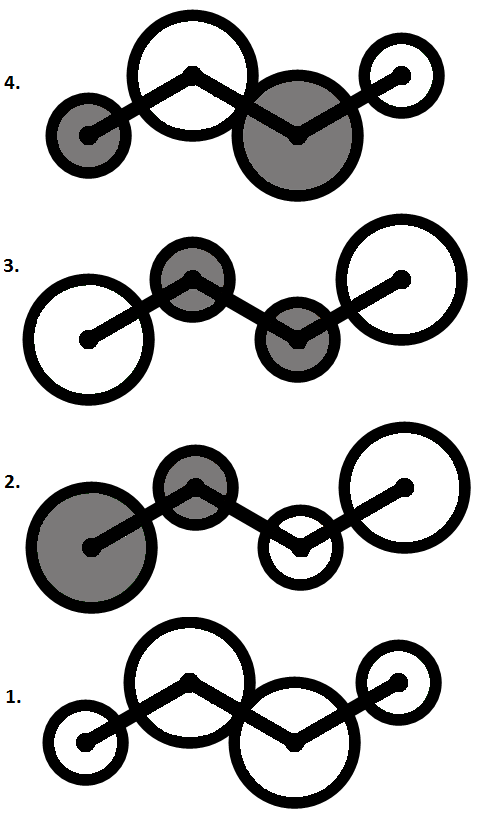
\includegraphics[width=\columnwidth]{pics/Hueckel_Butadiene.png}
 \caption{Aufsicht auf ein 1,3-Butadienmolekül. Schematische Darstellung der Hückelmolekülorbitale von 1,3-Butadien.}
 \label{fig:Hueckel_Butadiene}
\end{dsafigure}

Die Radien der Kreise entsprechen den Koeffizienten $c_{ik}$, während Weiß und Grau die Positivteile beziehungsweise Negativteile beschreiben. Das erste Orbital ist das energetisch günstigste Molekülorbital von Butadien, da es nur bindende Wechselwirkungen aufweist und keine Knotenebene besitzt; es ist ein bindendes Orbital. Das zweite Orbital hingegen weist zwei bindende Wechselwirkungen und eine Knotenebene auf. Es handelt sich auch hier um ein bindendes Orbital. Beim dritten un vierten Orbital handelt es sich um antibindende Orbitale. Das dritte Orbital zeigt zwei Knotenebenen und eine bindende Wechselwirkung und das vierte Orbital weist drei Knotenebenen und keine bindenden Wechselwirkungen auf. Sie haben also mehr Knotenebenen als bindende Wechselwirkungen. Die Energie vier Molekülorbitale nimmt in aufsteigender Reihenfolge zu.
